%%%%%%%%%%%%%%%%%%%%%%%%%%%%%%%%%%%%%%%%%%%%%%%%%%%%%%%%%%%%%%%%%%%%%%%%%%%%%%%%
%2345678901234567890123456789012345678901234567890123456789012345678901234567890
%        1         2         3         4         5         6         7         8

\documentclass[letterpaper, 10 pt, conference]{ieeeconf}  % Comment this line out
                                                          % if you need a4paper
%\documentclass[a4paper, 10pt, conference]{ieeeconf}      % Use this line for a4
                                                          % paper

\IEEEoverridecommandlockouts                              % This command is only
                                                          % needed if you want to
                                                          % use the \thanks command
\overrideIEEEmargins
% See the \addtolength command later in the file to balance the column lengths
% on the last page of the document



% The following packages can be found on http:\\www.ctan.org
\usepackage{graphics} % for pdf, bitmapped graphics files
\usepackage{epsfig} % for postscript graphics files
\usepackage{mathptmx} % assumes new font selection scheme installed
\usepackage{times} % assumes new font selection scheme installed
\usepackage{amsmath} % assumes amsmath package installed
\usepackage{amssymb}  % assumes amsmath package installed
\usepackage{graphicx}
\usepackage{float}
\usepackage[english,ngerman]{babel}
\usepackage{algpseudocode,amsmath}
\usepackage[linesnumbered,ruled]{algorithm2e}
\usepackage{algorithmicx}
\usepackage[section]{placeins}
\title{\LARGE \bf
Simulation On Creation Of Solar System
}

%\author{ \parbox{3 in}{\centering Huibert Kwakernaak*
%         \thanks{*Use the $\backslash$thanks command to put information here}\\
%         Faculty of Electrical Engineering, Mathematics and Computer Science\\
%         University of Twente\\
%         7500 AE Enschede, The Netherlands\\
%         {\tt\small h.kwakernaak@autsubmit.com}}
%         \hspace*{ 0.5 in}
%         \parbox{3 in}{ \centering Pradeep Misra**
%         \thanks{**The footnote marks may be inserted manually}\\
%        Department of Electrical Engineering \\
%         Wright State University\\
%         Dayton, OH 45435, USA\\
%         {\tt\small pmisra@cs.wright.edu}}
%}

\author{Rutvik N, Ramesh Chandra, Gourav Roy, Shashidhar G Koolagudi and Fathima Afroz\\ Dept. of Computer Science and Engineering\\ National Institute of Technology Karnataka\\ rutvikniranjan@gmail.com, rameshc10695@gmail.com, robrayneon@gmail.com
}


\begin{document}



\maketitle
\thispagestyle{empty}
\pagestyle{empty}


%%%%%%%%%%%%%%%%%%%%%%%%%%%%%%%%%%%%%%%%%%%%%%%%%%%%%%%%%%%%%%%%%%%%%%%%%%%%%%%%
\begin{abstract}
The formation of the solar system is a complicated and an interesting theory. Thereby, it has to be researched more in order to understand it better. The easiest way to understand is to visually see it happen. This paper uses graphics concepts to simulate the theories provided by various researchers on the formation of the solar system. The simulation is based on thorough and exhaustive research. The results provide a way to further the research and work on the evolution of the solar system.    

\end{abstract}


%%%%%%%%%%%%%%%%%%%%%%%%%%%%%%%%%%%%%%%%%%%%%%%%%%%%%%%%%%%%%%%%%%%%%%%%%%%%%%%%
\section{INTRODUCTION}
The creation of the Solar System began some 4.6 billion years ago when a small part of a giant molecular cloud collapsed due to gravitational effect.[1] Majority of the collapsing mass assembled in the middle, forming the Sun, while the remaining part flattened into a disk out of which the planets, moons, asteroids, and other small Solar System bodies were created.

This famously known mode, the nebular hypothesis, was initially developed in the 18th century by Emanuel Swedenborg, Immanuel Kant, and Pierre-Simon Laplace. Then the development has interwoven various scientific disciplines that include astronomy, physics, geology, and planetary science. Ever since the beginning of the space age in the 1950s and the discovery of extrasolar planets in the 1990s, the model has been both confronted and filtered to account for new observations.

In about 5 billion years, the Sun will cool and expand outward many more times its present diameter (red giant), then it will cast off its outer layers as a planetary nebula and then leave behind a stellar remainder, the white dwarf. Many more years later, the gravitational force of passing stars will slowly cut down the Sun's retinue of planets. Few planets will be annihilated, others discharged into the interstellar space. Eventually, over the course of time, about tens of billions of years, it is probable that the Sun will be left with none of the current bodies.[3]

The graphical components used to set up the simulation are opengl functions included in glew and glut libraries with a circle drawing algorithm developed by using triangle vertex method. The simulation consists mainly of three stages, the first being that of the giant cloud of gas which consisted of the particles responsible for creation of the solar system, the second one shows the giant ball formation at the center and the moving debris around it and the final one shows the last form of the solar system showing the orbiting of the planets, moons, asteroids and every other body that either revolves around the sun or any other planet of the solar system.

The purpose is pretty clear given the above introduction that it will mainly be used for educational purposes. Education in a more interactive way than any other. This document contains exhaustive information regarding the formation of the solar system. This document could be furthered by considering the evolution of the solar system and also talk about its predicted future. The proposed functions can be taken up by developers to further the development of the models and show the future of the solar system graphically.

This paper first presents a literature survey, talking about various theories that tell us about the formation and the evolution of the solar system. After getting a thorough insight of how the solar system was formed, we move on to approach and methodology. After understanding the exact approach and the algorithm, we move to the pseudo code where we shed light upon the implementation. We later move on to the results and the conclusion.



\section{Literature Survey}
Among the scientific investigations concerning the formation and evolution of the solar system, the main focus is on the planet formation, their orbit and how they came to be in that orbit, especially the path they take[6][9][19]. The hypothesis that solar was formed due to the explosion of a giant cloud of gas[9].  The further collapse of the fragments led to the formation of dense cores 0.01–0.1 pc (2,000–20,000 AU) in size.[9][11]. The most important criticism of the hypothesis was its inability to explain the Sun's relatively less amount of angular momentum when compared to other planets.[5]. The nuclear fusion which is the sun’s main source of energy and how does it affect the planets[7], that is the formation of helium from hydrogen items and other elements constituting the solar system[8], the chemistry and how they actually affect the system in general. The nebular theory [10], the nebula’s chemical composition [12] and its effect on the current form of the solar system actually provides a great insight on how the solar system reshaped itself into the current form. The future of the current system [17][18][19][20].


\section{APPROACH AND METHODOLGY}
The approach to this theory is to first divide the whole theory into three parts.
1. Cloud of gas with explosions happening due to which a bigger ball is formed at the center and the debris around it.
2. The sun and then the debris. Also, the grouping of certain set of debris leading to the actual formation of the planets.
3. The solar system itself, with the actual orbits  of the planets around the sun with their respective speeds, following their respective paths and also the satellites and all other debris between any set of planets.

The method to the above given approach is that we use the glut, math and time libraries to help us get across to implement the above proposed approach. The chart below shows the steps we need to completely demonstrate the process.
\begin{figure}[H]
  \begin{center}
    \includegraphics[width=8cm]{_1.png}
  \end{center}
  \caption{Phase 1. Cloud of gas with internal explosions.}
\end{figure}


\begin{figure}[H]
  \begin{center}
    \includegraphics[width=8cm]{_2.png}
  \end{center}
  \caption{Phase 2. The sun with debris movement and the grouping of certain specific sets of debris.}
\end{figure}

\begin{figure}[H]
  \begin{center}
    \includegraphics[width=8cm]{_3.png}
  \end{center}
  \caption{Phase 3. The solar system itself along with the actual orbits.}
\end{figure}
\section{IMPLEMNTATION}
The design and implementation of the above given methodology/algorithm mainly comes from the use of the functions from the glut, math and time libraries. The following will be a list of pseudocodes required in the implementation. The challenge lies in writing the algorithm based on the actual physical laws followed by the solar system. Due to the extensive research done by our fellow men it is easier for us to understand what really happened and come up with an algorithm that could actually simulate the formation of the solar system.
\algdef{SE}[DOWHILE]{Do}{doWhile}{\algorithmicdo}[1]{\algorithmicwhile\ #1}%

\subsection{Phase 1}
     \begin{algorithmic}
     \State $ x \leftarrow 0 $\;
  \Do
    \State glTranslatef (0.0, 0.0, -10.0)\;
  	\State	glRotatef (angle, 1.0, 1.0, 1.0)\;
     \State 		glScalef(1.0,x,1.0+1-x)\;
     \State 	glutSolidSphere(2,20,20)\;
	\State $ x \leftarrow x+0.1 $\;
  \doWhile{$x \leq 1$} % <--- use \doWhile for the "while" at the end
\end{algorithmic}

\subsection{Phase 2}
\begin{algorithmic}\State $ x \leftarrow 0 $\;

\Do 
       \State  glutSolidSphere(1.0,20,20)\;
      	\State	glScalef(1.0,x,1.0)\;
      	\State $ x \leftarrow x+0.1 $\;
\doWhile{ $x \leq 1$} \\

\end{algorithmic}
    
 \begin{algorithmic}
 \State $ z \leftarrow 1.5 $\;
\Do 
    \State $ a \leftarrow 0 $\;
    \Do 		
			\State drawHollowCircle(0.0, 0.0, z+y*a)\;
 			\State drawHollowCircle(0.0, 0.0, z-y*a)\;
 			\State $ a \leftarrow a+1 $\;
	\doWhile {$ a \leq 5$ }
        \State $ z \leftarrow z+0.5 $\;
\doWhile{ $z \leq 4$} \\
\end{algorithmic}
\subsection{Phase 3}

\begin{algorithmic}
\Function{drawplanet}{\null} 
\State		glColor3f(1.0f, 1.0f, 0.0f)\;
\State		glTranslatef(0.0f ,0.75f, 0.0f) \;
  \State  glutSolidSphere(3.0f,100,100) \;
  \State glEnd() \;
\EndFunction
\end{algorithmic}


%\begin{algorithmic}
%\Function {zoomfunction}{}
%\State		\Switch (key) \;
%\State		\hspace*{5mm}	\case $GLUT\_KEY\_LEFT$ :\;
%\State				$angle \leftarrow angle+ 0.01f$\;
%\State				$lx \leftarrow sin(angle)$\;
%\State				$lz \leftarrow -cos(angle) $\;
%\State			break\;
%\State			\case $GLUT\_KEY\_RIGHT$ : \;
%\State				$lx \leftarrow sin(angle) $ \;
%\State				$lz \leftarrow -cos(angle) $ \;
%\State				break\;
%\State			\case $GLUT\_KEY\_UP$ :\;
%\State				$x \leftarrow x+ lx * fraction $\;
%\State				$z \leftarrow z+ lz * fraction $\;
%\State				break\;
%\State		\case $GLUT\_KEY\_DOWN$ :\;
%\State			$x \leftarrow x+lx * fraction $\;
%\State			$ z \leftarrow z+ lz * 	fraction $ \;
%\State	        break\;
%\EndFunction
%\end{algorithmic}

	\hspace*{5mm} \textbf{function} zoomfunction() \\
\hspace*{10mm}		switch (key) \\
\hspace*{15mm}			case $GLUT\_KEY\_LEFT$ :\\
\hspace*{20mm}				$angle \leftarrow angle+ 0.01f$;\\
\hspace*{20mm}				$lx \leftarrow sin(angle)$;\\
\hspace*{20mm}				$lz \leftarrow -cos(angle) $;\\
	\hspace*{15mm}			break;\\
\hspace*{15mm}			case $GLUT\_KEY\_RIGHT$ : \\
\hspace*{20mm}			$	angle \leftarrow angle +0.01f $; \\
\hspace*{20mm}				$lx \leftarrow sin(angle) $; \\
\hspace*{20mm}				$lz \leftarrow -cos(angle) $; \\
\hspace*{15mm}				break;\\
\hspace*{15mm}			case $GLUT\_KEY\_UP$ :\\
\hspace*{20mm}				$x \leftarrow x+ lx * fraction $;\\
\hspace*{20mm}				$z \leftarrow z+ lz * fraction $;\\
\hspace*{15mm}				break;\\
\hspace*{15mm}			case $GLUT\_KEY\_DOWN$ :\\
\hspace*{20mm}			$x \leftarrow x+lx * fraction $;\\
\hspace*{20mm}			$ z \leftarrow z+ lz * 	fraction $ ;\\
\hspace*{15mm}				break; \\ \\ 
\hspace*{5mm} \textbf{end function}
\begin{algorithmic}
\Function{drawStar}{\null} 
\State		glColor3f(1.0f, 1.0f, 1.0f) \;
\State		glBegin($GL\_POINTS$) \;
  \State  		glVertex3f(-10.0f, -3.0f, 0.0f) \;
  \State glEnd() \;
\EndFunction
\end{algorithmic}

\subsection{Other functions that need to be used}

\begin{itemize}
\item  glEnable($ GL\_BLEND $); - After blending is enabled, as shown above, the incoming primitive color is blended with the color already stored in the framebuffer. glBlendFunc () controls how this blending occurs. The typical use described above modifies the incoming color by its associated alpha value and modifies the destination color by one minus the incoming alpha value. The sum of these two colors is then written back into the framebuffer.
\item  glEnable ($ GL\_LIGHTING $);- OpenGL approximates light and lighting as if light can be broken into red, green, and blue components. Thus, the color of light sources is characterized by the amount of red, green, and blue light they emit, and the material of surfaces is characterized by the percentage of the incoming red, green, and blue components that is reflected in various directions. The OpenGL lighting equations are just an approximation but one that works fairly well and can be computed relatively quickly.
\item glEnable ($ GL\_LIGHT0 $);- Like lights, materials have different ambient, diffuse, and specular colors, which determine the ambient, diffuse, and specular reflectances of the material. A material's ambient reflectance is combined with the ambient component of each incoming light source, the diffuse reflectance with the light's diffuse component, and similarly for the specular reflectance and component. Ambient and diffuse reflectance’s define the color of the material and are typically similar if not identical. Specular reflectance is usually white or gray, so that specular highlights end up being the color of the light source's specular intensity. If you think of a white light shining on a shiny red plastic sphere, most of the sphere appears red, but the shiny highlight is white
\item glPushMatrix($ $); glPopMatrix (); - There is a stack of matrices for each of the matrix modes. In $ GL_MODELVIEWmode $, the stack depth is at least 32. In the other modes,$GL\_COLOR$,$GL\_PROJECTION$, and $GL\_TEXTURE$, the depth is at least 2. The current matrix in any mode is the matrix on the top of the stack for that mode.
\item glTranslatef($ $)- glTranslate produces a translation by x y z . The current matrix (see glMatrixMode) is multiplied by this translation matrix, with the product replacing the current matrix, as if glMultMatrix were called with the following matrix for its argument:  1 0 0 x 0 1 0 y 0 0 1 z 0 0 0 1If the matrix mode is either $GL\_MODELVIEW$ or $GL\_PROJECTION$, all objects drawn after a call to glTranslate are translated. Use  glPushMatrix and glPopMatrix to save and restore the untranslated coordinate system.
\item glRotatef($ $)   - glRotateproduces a rotation ofangledegrees around the vector[x][y][z]
\item  glutSolidSphere -for sphere creation.
\item  glColor3f -for coloring.

\end{itemize}

\section{Result}

\begin{figure}[H]
  \begin{center}
    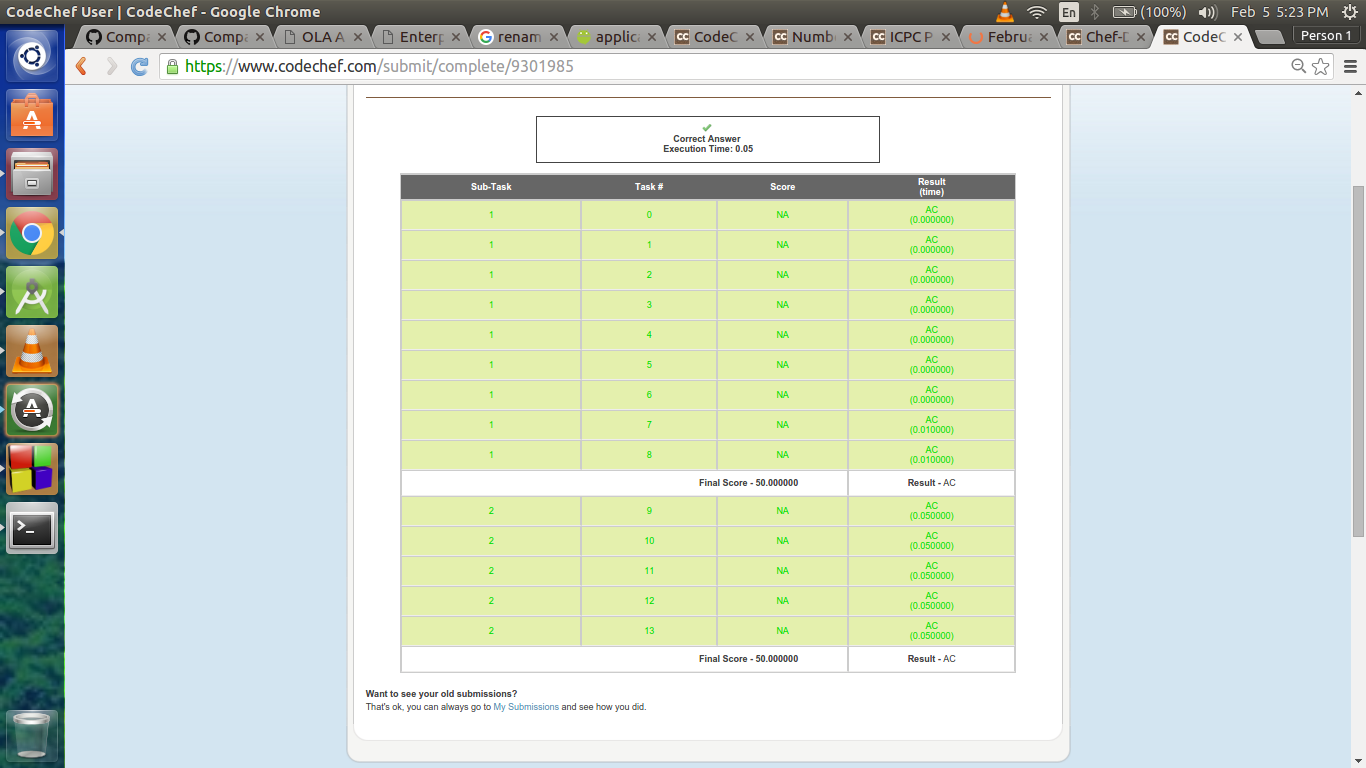
\includegraphics[width=8cm]{1.png}
  \end{center}
  \caption{Shows the phase 1 of the project with \newline expanding sphere of particles}
\end{figure}

\begin{figure}[H]
  \begin{center}
    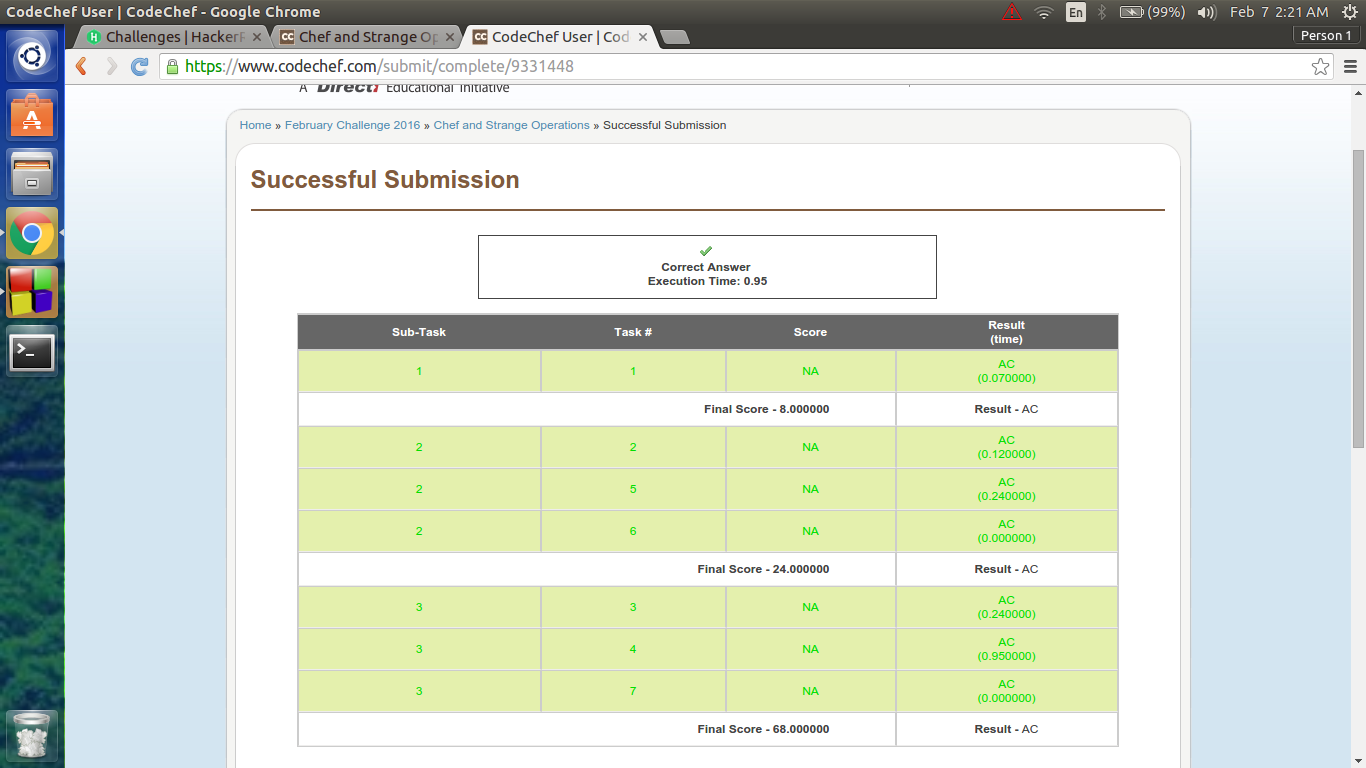
\includegraphics[width=8cm]{2.png}
  \end{center}
  \caption{Phase 2 of the simulation where the disk  like structures are formed around sun}
\end{figure}
\begin{figure}[H]
  \begin{center}
    \includegraphics[width=8cm]{3.png}
  \end{center}
  \caption{the 3rd phase of the simulation showing the \newline complete solar system with the first 5 planets}
\end{figure}



\section{CONCLUSION}
Researchers have spent many years trying to understand the solar system leave alone the evolution of it. The evolution of this system is quite complicated and interesting. After researching a lot, it was easier to implement and understand the working of the solar system and how it came into being. This research and the document can be used for further research on this topic. This can be used by developers for further development of the evolution of the solar system. Of course the main aim of this document is to provide an insight into the formation of the solar system graphically. With an ever changing technology in this world, everyday a better software is available as far as graphics is concerned. The use of new technology will further improve the quality of the projects we can do as graphics researchers. The three phase system presented above is an effective and efficient way of showing the actual formation of the solar system. The three phase division is especially useful to easily understand and demonstrate. 
\section{FUTURE WORK}
Astronomers predict that the Solar System will not change until the Sun has fused almost all hydrogen fuel in its core into helium after that it will move from current phase to red-giant phase. The Solar System is chaotic over million- and billion-years and the orbits of the planets open to long-term changes. Ultimately, no major changes will take place until next few billion years. After that, within five billion years Mars's eccentricity may grow to approx. 0.2, such that it lies on an Earth-crossing orbit, leading to a probable collision. Mercury's eccentricity may grow even further, and a collision with Venus could theoretically remove it from the Solar System altogether.

Sun will start combustion of hydrogen in a shell encapsulating its core, ending the main sequence life. Sun shall then begin to ascend the red giant sequence, growing dramatically more luminous (by a factor of up to 2,700), larger (by a factor of up to 250 in radius), and cooler (down to 2600 K). Mercury, Venus and Earth are swallowed. Saturn's moon Titan shall become habitable. Sun goes through helium burning horizontal branch and giant branch phases, losing approx. 30\% of its mass in all post main sequence phases. The giant phase ends with the removal of a planetary nebula, leading to the formation of a white dwarf. Sun cools down to 5 K. Gravity of many closely moving stars shall detach planets from orbits. Solar System will cease to exist. Our future work shall be to implement to above given two paragraphs.


\addtolength{\textheight}{-12cm}   % This command serves to balance the column lengths
                                  % on the last page of the document manually. It shortens
                                  % the textheight of the last page by a suitable amount.
                                  % This command does not take effect until the next page
                                  % so it should come on the page before the last. Make
                                  % sure that you do not shorten the textheight too much.

%%%%%%%%%%%%%%%%%%%%%%%%%%%%%%%%%%%%%%%%%%%%%%%%%%%%%%%%%%%%%%%%%%%%%%%%%%%%%%%%



%%%%%%%%%%%%%%%%%%%%%%%%%%%%%%%%%%%%%%%%%%%%%%%%%%%%%%%%%%%%%%%%%%%%%%%%%%%%%%%%



%%%%%%%%%%%%%%%%%%%%%%%%%%%%%%%%%%%%%%%%%%%%%%%%%%%%%%%%%%%%%%%%%%%%%%%%%%%%%%%%

%%%%%%%%%%%%%%%%%%%%%%%%%%%%%%%%%%%%%%%%%%%%%%%%%%%%%%%%%%%%%%%%%%%%%%%%%%%%%%%%

References are important to the reader; therefore, each citation must be complete and correct. If at all possible, references should be commonly available publications.



\begin{thebibliography}{99}
\bibitem{c1}Audrey Bouvier, Meenakshi Wadhwa (2010). "The age of the solar system redefined by the oldest Pb-Pb age of a meteoritic inclusion". Nature Geoscience 3: 637–641.Bibcode:2010NatGe...3..637B. doi:10.1038/NGEO941.
\bibitem{c2}Gomes, R.; Levison, Harold F.; Tsiganis, K.; Morbidelli, Alessandro (2005)."Origin of the cataclysmic Late Heavy Bombardment period of the terrestrial planets"(PDF). Nature 435 (7041): 466–9
\bibitem{c3}Freeman Dyson (July 1979). "Time Without End: Physics and Biology in an open universe". Reviews of Modern Physics (Institute for Advanced Study, Princeton New Jersey) 51 (3): 447–460. Bibcode:1979RvMP...51..447D.
\bibitem{c4}Jane S. Greaves (2005). "Disks Around Stars and the Growth of Planetary Systems".Science
\bibitem{c5}M. M. Woolfson (1984). "Rotation in the Solar System". Philosophical Transactions of the Royal Society 313 (1524): 5–18.
\bibitem{c6}Nigel Henbest (1991). "Birth of the planets: The Earth and its fellow planets may be survivors from a time when planets ricocheted around the Sun like ball bearings on a pinball table".
\bibitem{c7}David Whitehouse (2005). The Sun: A Biography. John Wiley and Sons
\bibitem{c8}Simon Mitton (2005). "Origin of the Chemical Elements". Fred Hoyle: A Life in Science. Aurum. pp. 197–222.
\bibitem{c9}Thierry Montmerle, Jean-Charles Augereau, Marc Chaussidon (2006). "Solar System Formation and Early Evolution: the First 100 Million Years". Earth, Moon, and Planets (Spinger) 98 (1–4): 39–95.
\bibitem{c10}Ann Zabludoff (University of Arizona) (Spring 2003). "Lecture 13: The Nebular Theory of the origin of the Solar System". Retrieved 2006-12-27.
\bibitem{c11}J. J. Rawal (1986). "Further Considerations on Contracting Solar Nebula" (PDF).Earth, Moon, and Planets (Nehru Planetarium, Bombay India: Springer Netherlands) 34 (1): 93–100.
\bibitem{c12}W. M. Irvine (1983). "The chemical composition of the pre-solar nebula". In T. I. Gombosi (ed.). Cometary Exploration.
\bibitem{c13}Caffe, M. W.; Hohenberg, C. M.; Swindle, T. D.; Goswami, J. N. (February 1, 1987). "Evidence in meteorites for an active early sun".
\bibitem{c14}Charles H. Lineweaver (2001). "An Estimate of the Age Distribution of Terrestrial Planets in the Universe: Quantifying Metallicity as a Selection Effect". Icarus 151 (2): 307–313.
\bibitem{c15}Williams, J. (2010). "The astrophysical environment of the solar birthplace".
\bibitem{c16}J. Jeff Hester, Steven J. Desch, Kevin R. Healy, Laurie A. Leshin (21 May 2004). "The Cradle of the Solar System".
\bibitem{c17}Martin Bizzarro, David Ulfbeck, Anne Trinquier, Kristine Thrane, James N. Connelly, Bradley S. Meyer (2007). "Evidence for a Late Supernova Injection of 60Fe into the Protoplanetary Disk"
\bibitem{c18}Morgan Kelly. "Slow-Moving Rocks Better Odds That Life Crashed to Earth from Space"
\bibitem{c19}Simon F. Portegies Zwart (2009). "The Lost Siblings of the Sun". Astrophysical Journal696 (L13–L16): L13. arXiv:0903.0237
\bibitem{c20}Nathan A. Kaib and Thomas Quinn (2008). "The formation of the Oort cloud in open cluster environments"

\end{thebibliography}




\end{document}

